\chapter*{9. laboratorijska naloga}
\section*{Realizacija konènih avtomatov s pomnilnimi celicami\\(Moorov avtomat)}

Z uporabo logiènih vrat in pomnilnih celic želimo realizirati Moorov avtomat. Postpek realizacije je sestavljen iz sledeèih korakov:
\begin{enumerate}
\item \emph{Zapis kodirnih tabel}: vhodna abeceda, notranja abeceda in izhodna abeceda so predstavljene z abstraktnim zapisom. Za realizacijo s preklopnimi funkcijami moramo le-te predstaviti s preklopnimi spremenljivkami. Pri tem upoštevamo dejstvo, da lahko z $n$ vhodnimi spremenljivkami zakodiramo bodisi $2^n$ vhodnih èrk ali $2^n$ izhodnih èrk, z $n$ pomnilnimi celicami pa $2^n$ notranjih stanj. S kodiranimi tabelami povežemo posamezne spremenljivke/pomnilne celice s posameznimi èrkami oziroma stanji avtomata.
\item \emph{Zapis pravilnostne tabele avtomata}: na podlagi diagrama prehajanja stanj oziroma tabele prehajanja stanj in kodirnih tabel, lahko zapišemo pravilnostno tabelo avtomata. Pri tem na levi strani tabele nastopajo spremenljivke, ki doloèajo vhodne èrke in trenutna notranja stanja (neodvisne spremenljivke), na desni strani pa spremenljivke, ki doloèajo notranje stanje avtomata v naslednjem èasovnem koraku in spremenljivke, ki doloèajo izhodne izhodne èrke avtomata (odvisne spremenljivke).
\item \emph{Doloèitev vhodov v pomnilne celice}: na podlagi prehodov med spremenljivkami, ki doloèajo trenutno stanje avtomata in stanje avtomata v naslednjem èasovnem koraku ter razpoložljivih pomnilnih celic, lahko doloèimo potrebne vhode v pomnilne celice v posamezni vrstici (tabelo dopolnimo na podoben naèin kot smo jo pri realizaciji sekvenènih vezij s pomnilnimi celicami). 
\item \emph{Doloèitev izhodne funkcije in funkcije prehajanja stanj}: na podlagi pravilnostne tabele lahko s pomoèjo Veitchevega diagrama izpišemo preklopne funkcije, ki doloèajo izhodne èrke avtomata (izhodna funkcija) in preklopne funkcije, ki nastopajo na vhodih pomnilnih celic in tako doloèajo prehode med stanji avtomata (funkcija prehajanja stanj)
\end{enumerate}

\begin{zgled}

Z uporavo T pomnilnih celic in poljubnimi logiènimi vrati realiziraj Moorov avtomat, ki je podan z diagramom prehajanja stanj.

\begin{center}
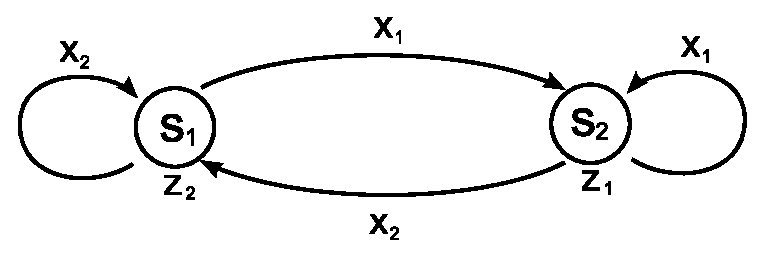
\includegraphics[width=0.5\linewidth]{slika_v10_1.eps}
\end{center}

\bigskip

\begin{enumerate} 

\item Zapišemo kodirne tabele, ki doloèijo kodiranje vhodne abecede, notranjih stanj in izhodne abecede. Za zapis vseh èrk v vhodne abecede je dovolj 1 vhodna spremenljivka ($x$); prav tako za zapis vseh èrk izhodne abecede ($y$). Ker imamo zgolj dve notranji stanji avtomatsa, je za njegovo realizacijo potrebna 1 pomnilna celica T z notranjim stanjem $q$. Kodirne tabele so torej

\begin{table}[ht]
\begin{center}
\begin{tabular}{ccc}
	\begin{tabular}{c|c}
	 & $x$ \\ 
		\hline
		$x_1$ & $0$\\
		$x_2$ & $1$\\
	\end{tabular}
	&
	\begin{tabular}{c|c}
		 & $q$ \\ 
		\hline
		$S_1$ & $0$\\
		$S_2$ & $1$\\
	\end{tabular}
	&
	\begin{tabular}{c|c}
		 & $z$ \\ 
		\hline
		$z_1$ & $0$\\
		$z_2$ & $1$\\
	\end{tabular}
\end{tabular}
\end{center}
\end{table}

\end{enumerate}

\item Na podlagi kodirnih tabel in podanega diagrama prehajanja stanj lahko zapišemo pravilnostno tabelo avtomata. Pri tem v levi strani tabele nastopajo spremenljivke, ki doloèajo trenutno notranje stanje avtomata ($q$) in vhodno èrko ($x$), na desni pa spremenljivke, ki doloèajo notranje stanje avtomata v naslednjem èasovnem koraku ($D^1q$) in izhodno èrko ($z$):

\begin{center}
\begin{tabular}{cc|cc}
 $q$ & $x$ & $D^1 q$ & $z$\\
 \hline
 0 & 0 & 1 & 1\\		 
 0 & 1 & 0 & 1\\
 1 & 0 & 1 & 0\\
 1 & 1 & 0 & 0\\
\end{tabular}
\end{center}

\item Na podlagi prehodov med spremenljivkami $q$ in $D^1q$ in tabele prehodov za T pomnilno celico, lahko doloèimo vrednosti, ki morajo biti na vhodu $t$ pri posamezni kombinaciji vhodnih spremenljivk:

\begin{center}
\begin{tabular}{cc|cc|c}
 $q$ & $x$ & $D^1 q$ & $z$ & $t$\\
 \hline
 0 & 0 & 1 & 1 & 1 \\		 
 0 & 1 & 0 & 1 & 0 \\
 1 & 0 & 1 & 0 & 0 \\
 1 & 1 & 0 & 0 & 1 \\
\end{tabular}
\end{center}



\item Na podlagi pravilnostne tabele lahko s pomoèjo Veitchevega diagrama izpišemo preklopno funkcijo izhodne èrke avtomata in preklopno funkcijo, ki nastopajo na vhodu T pomnilne celice:


\begin{figure}[!ht]
\begin{center}
\begin{tabular}{cc}
\begin{tabular}{|c|c|}
\hline
1 & 0 \\
\hline
0 & 1\\
\hline
\end{tabular} &
\begin{tabular}{|c|c|}
\hline
0 & 1 \\
\hline
0 & 1\\
\hline
\end{tabular} \\
$t = \ol x \ol q \vee x q = x \equiv q$ & $z = \ol q$\\
\end{tabular}
\end{center}
\end{figure}


Èe funkcijo na vhodu T pomnilne celice vstavimo v enaèbo T pomnilne celice ($D^1 q = t \ol q \vee \ol t q$), dobimo \emph{funkcijo prehajanja stanj} avtomata:
$$
D^1q = (x \equiv q) \ol q \vee \ol{(x \equiv q)} q = (x \equiv q) \ol q \vee (x \nabla q) q 
$$ 

Po definiciji velja, da je izhodna èrka Moorovega avtomata doloèena s trenutnim stanjem avtomata. Velja torej, da je izhodno èrko pri Moorovem avtomatu vedno mogoèe izraziti zgolj s spremenljivkami, ki doloèajo trenutno stanje avtomata ($q$).


\subsubsection{Realizacija Mealyjevega avtomata}

S tabelo prehajanja stanj je podan Mealyjev avtomat:

\bigskip

\begin{tabular}{c|ccc}
 & $S_1$ & $S_2$ & $S_3$\\
\hline
$x_1$ & $S_2 / z_1$ & $S_2 / z_2$ & $S_1 / z_1$\\
$x_2$ & $S_1 / z_2$ & $S_3 / z_1$ & $S_3/ z_2$ \\
\end{tabular}

\bigskip

Želimo ga realizirati s T pomnilnimi celicami.

\bigskip

Zapišemo kodirne tabele. Ker imamo tri notranja stanja, jih zakodiramo z dvema bitoma:

\bigskip

\begin{tabular}{c|c}
 & $x$ \\ 
\hline
$x_1$ & $0$\\
$x_2$ & $1$\\
\end{tabular}

\bigskip

\begin{tabular}{c|cc}
 & $q_1$ & $q_2$ \\ 
\hline
$S_1$ & $0$ & $0$\\
$S_2$ & $0$ & $1$\\
$S_3$ & $1$ & $0$\\
\end{tabular}

\bigskip

\begin{tabular}{c|c}
 & $z$ \\ 
\hline
$z_1$ & $0$\\
$z_2$ & $1$\\
\end{tabular}

\bigskip

Za realizacijo avtomata bomo torej potrebovali 2 pomnilni celici.

\bigskip

Na podlagi kodirnih tabel in podane tabele prehajanja stanj lahko zapišemo pravilnostno tabelo avtomata in doloèimo vrednosti vhodov v T pomnilni celici pri posamezni kombinaciji vhodnih spremenljivk:

\bigskip

\begin{tabular}{ccc|ccc|cc}
 $q_1$ & $q_2$ & $x$ & $D^1 q_1$ & $D^1 q_2$ & $z$ & $t_1$ & $t_2$\\
  \hline
 0 & 0 & 0 & 0 & 1 & 0 & 0 & 1\\		 
 0 & 0 & 1 & 0 & 0 & 1 & 0 & 0\\		 
 0 & 1 & 0 & 0 & 1 & 1 & 0 & 0\\		 
 0 & 1 & 1 & 1 & 0 & 0 & 1 & 1\\		 
 1 & 0 & 0 & 0 & 0 & 0 & 1 & 0\\		 
 1 & 0 & 1 & 1 & 0 & 1 & 0 & 0\\		 
 1 & 1 & 0 & ? & ? & ? & ? & ?\\		 
 1 & 1 & 1 & ? & ? & ? & ? & ?\\		 
\end{tabular}

\bigskip

S pomoèjo Veitchevega diagram doloèimo preklopno funkcijo vhoda v T pomnilni celici:

\bigskip
$t_1$:
\begin{tabular}{|c|c|c|c|}
\hline
? & ? & 1 & 0 \\
\hline
1 & 0 & 0 & 0\\
\hline
\end{tabular}

$$
t_1 = q_1 \ol x \vee q_2 x
$$

\bigskip
$t_2$:
\begin{tabular}{|c|c|c|c|}
\hline
? & ? & 1 & 0 \\
\hline
0 & 0 & 0 & 1\\
\hline
\end{tabular}

$$
t_2 = x q_2 \vee \ol x \ol q_1 \ol q_2
$$

\bigskip

Z Veitchevim diagramom doloèimo še preklopno funkcijo izhodne èrke $z$:

\bigskip
$z$:
\begin{tabular}{|c|c|c|c|}
\hline
? & ? & 0 & 1 \\
\hline
0 & 1 & 1 & 0\\
\hline
\end{tabular}

$$
z = x \ol q_2 \vee \ol x q_2 = x \nabla q_2
$$

V tem primeru je izhodna èrka doloèena s trenutnim stanjem in z vhodno èrko avtomata.

\bigskip

\includegraphics[width=0.6\linewidth]{vaja10_02_main.eps} \\
\includegraphics[width=0.4\linewidth]{vaja10_02_t1.eps} \\
\includegraphics[width=0.4\linewidth]{vaja10_02_t2.eps} \\
\includegraphics[width=0.4\linewidth]{vaja10_02_z.eps} \\

\end{zgled}

\newpage

\section*{Laboratorijske vaje}
V Logisim-u z uporabo T pomnilnih celic realiziraj Moorov avtomat, podan s spodnjo tabelo.

\bigskip
\begin{center}
\large
\begin{tabular}{c|ccc}
& $z_1$ & $z_2$ & $z_3$\\
& $S_1$ & $S_2$ & $S_3$\\
\hline
$x_1$ & $S_1$ & $S_1$ & $S_1$\\
$x_2$ & $S_2$ & $S_3$ & $S_2$\\
\end{tabular}
\end{center}

\bigskip
Postopek:
\begin{enumerate}
\item Doloèi kodirne tabele.
\item Zapiši pravilnostno tabelo avtomata.
\item Doloèi funkcijo prehajanja notranjih stanj.
\item Doloèi izhodno funkcijo.
\item Realiziraj vezje v Logisimu.
\end{enumerate}

\bigskip
\textbf{REŠITEV.}

\bigskip
Kodirne tabele:

\bigskip
\begin{tabular}{c|c}
& $x$\\
\hline
$x_1$ & $0$\\
$x_2$ & $1$
\end{tabular}
\hspace{1cm}
\begin{tabular}{c|cc}
& $q_1$ & $q_2$\\
\hline
$S_1$ & $0$ & $0$\\
$S_2$ & $0$ & $1$\\
$S_3$ & $1$ & $0$
\end{tabular}
\hspace{1cm}
\begin{tabular}{c|cc}
& $y_1$ & $y_2$\\
\hline
$z_1$ & $0$ & $0$\\
$z_2$ & $0$ & $1$\\
$z_3$ & $1$ & $0$
\end{tabular}

\bigskip
Pravilnostna tabela avtomata:

\bigskip
\begin{tabular}{ccc|cccc|cc}
$q_1$ & $q_2$ & $x$ & $D^1 g_1$ & $D^1 g_2$ & $y_1$ & $y_2$ & $t_1$ & $t_2$\\
\hline
0 & 0 & 0 & 0 & 0 & 0 & 0 & 0 & 0\\
0 & 0 & 1 & 0 & 1 & 0 & 0 & 0 & 1\\
0 & 1 & 0 & 0 & 0 & 0 & 1 & 0 & 1\\
0 & 1 & 1 & 1 & 0 & 0 & 1 & 1 & 1\\
1 & 0 & 0 & 0 & 0 & 1 & 0 & 1 & 0\\
1 & 0 & 1 & 0 & 1 & 1 & 0 & 1 & 1\\
1 & 1 & 0 & ? & ? & ? & ? & ? & ?\\
1 & 1 & 1 & ? & ? & ? & ? & ? & ?\\
\end{tabular}

\bigskip
Funkcija prehajanja stanj:\\
$t_1(g_1, g_2, x) = g_1 \vee g_2 x$\\
$t_2(g_1, g_2, x) = q_2 \vee x$

\bigskip
Izhodna funkcija:\\
$y_1(q_1, q_2) = q_1$\\
$y_2(q_1, q_2) = q_2$
